\documentclass[default,pdf,colorBG,slideColor]{prosper}
\usepackage{epsfig}
\usepackage{pstricks}
\usepackage{graphicx}

\graphicspath{ {../fig/} }

\title{Next Generation Resource Manager}
\subtitle{{\small high level technical review}}
\author{Dong Ahn, Jim Garlick, Mark Grondona, Don Lipari}
\email{{\rm \{ahn1,garlick,mgrondona,lipari\}@llnl.gov}}
\institution{Livermore Computing \\
             Lawrence Livermore National Laboratory}

\newcommand{\ngrm}{NGRM}
\newcommand{\zMQ}{\O{}MQ}

\slideCaption{\ngrm\ High Level Review, Mar. 4, 2013}

\Logo(-1,-1){
\epsfig{file=graphic/iccd_logotrans.ps,scale=0.15}}

%\Logo{
\includegraphics[scale=0.15]{iccd_logotrans.ps}}

\newif\ifbigpic
\bigpictrue


\begin{document}

% ==========================================================================
\maketitle
% ==========================================================================
\begin{slide}{Session Overview}{\small
We will roughly follow the outline of the {\em Vision} document.\\
\begin{itemize}
  \item[\S1-4]{{\em overview} (Jim)}
  \item[\S5]{{\em comms framework} (Jim)}
  \item[\S6.1-6]{{\em resource management} (Mark)}
  \item[\S6.7]{{\em scheduler} (Don)}
  \item[\S7]{{\em monitoring} (Jim)}
  \item[\S8]{{\em runtime} (Dong)}
\end{itemize}
We expect to address your questions and comments as we go.
}\end{slide}
% ==========================================================================
\part{overview}
% ==========================================================================
\begin{slide}{RM today}{\small
Here describe slurm emphasising its design space, scalability
limitations, node-centric resource model, etc..  What is good about slurm
that we would like to carry fwd.
}\end{slide}
% ==========================================================================
\begin{slide}{vision and new capabilities}{\small
\begin{itemize}
  \item{center as a cluster}
  \item{diverse compute resources}
  \item{data provenance and reproduceability}
  \item{low noise}
  \item{fault tolerance}
  \item{security}
  \item{research and tool friendly}
  \item{extensibility}
\end{itemize}
}\end{slide}
% ==========================================================================
\begin{slide}{design challenges}{\small
\begin{minipage}{0.45\textwidth}
\begin{itemize}
  \item{multidimensional scale challenge}
  \item{diverse workload challenge}
  \item{dynamic workload challenge}
  \item{power challenge}
  \item{scheduling challenge}
\end{itemize}
\end{minipage}
\begin{minipage}{0.45\textwidth}
\begin{itemize}
  \item{backwards compatibility challenge}
  \item{integration risk}
  \item{higher downtime costs}
  \item{separation-of-concerns challenge}
  \item{security challenge}
  \item{productivity challenges}
\end{itemize}
\end{minipage}
}\end{slide}
% ==========================================================================
\begin{slide}{new conceptual models}{\small
\begin{itemize}
  \item{unified job model}
  \item{job hierarchy model}
  \item{generalized resource model}
  \item{resource allocation elasticity model}
  \item{common scalable infrastructure model}
  \item{self-hosting model}
  \item{lightweight virtualization model}
\end{itemize}
}\end{slide}
% ==========================================================================
\begin{slide}{Next Generation Resource Manager}{\small
insert {\em vision} figure 2 job hierarchy (several slides showing
progression.
}\end{slide}
% ==========================================================================
\begin{slide}{job 0}{\small
\ifbigpic
\begin{center}
  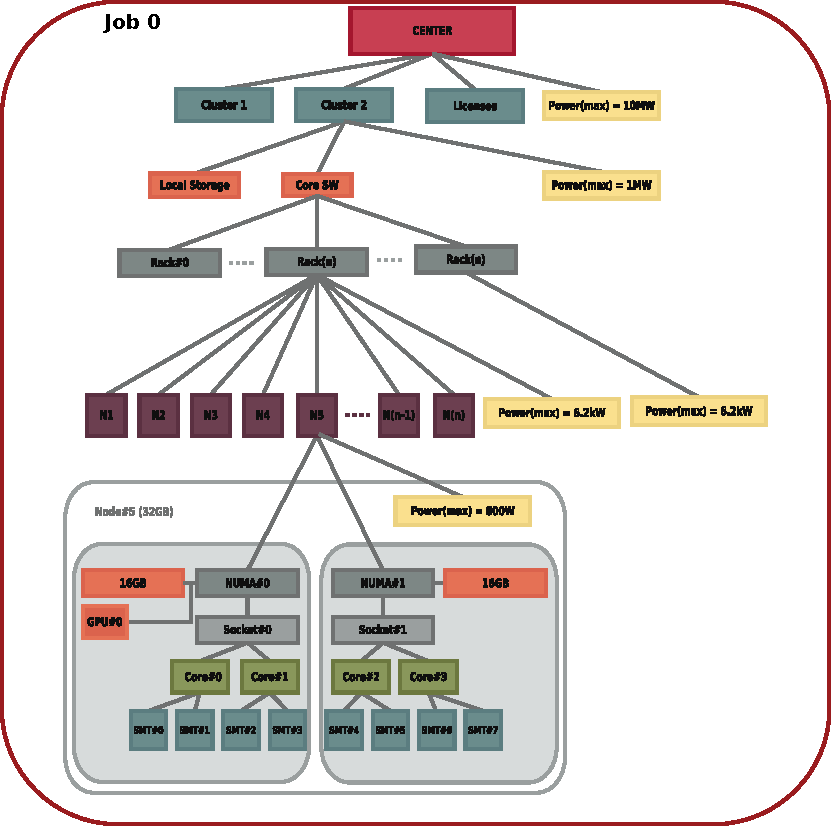
\includegraphics[scale=0.50]{job-hierarchy-job0}
\end{center}
\fi
}\end{slide}
% ==========================================================================
\begin{slide}{job 0.x}{\small
\ifbigpic
\begin{center}
  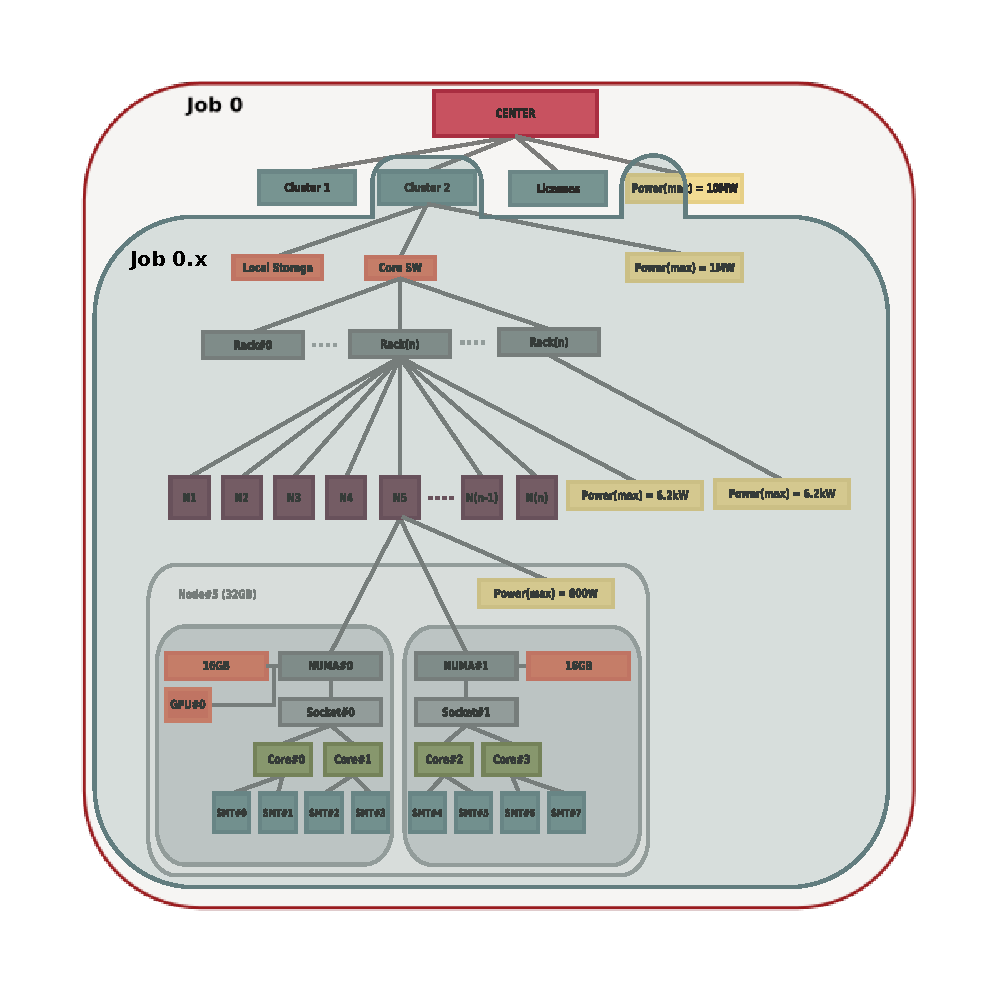
\includegraphics[scale=0.50]{job-hierarchy-job0-x}
\end{center}
\fi
}\end{slide}
% ==========================================================================
\begin{slide}{job 0.x.y}{\small
\ifbigpic
\begin{center}
  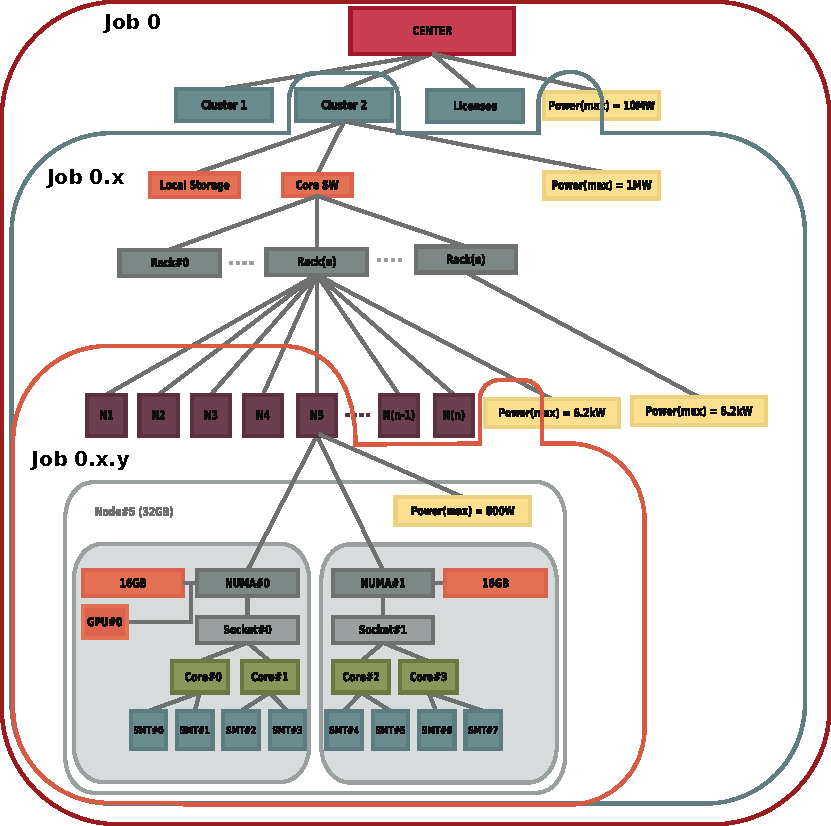
\includegraphics[scale=0.50]{job-hierarchy-job0-x-y}
\end{center}
\fi
}\end{slide}
% ==========================================================================
\begin{slide}{comparision with slurm}{\small
\begin{itemize}
  \item{job}
  \item{job step}
  \item{reservations}
  \item{job accounting}
\end{itemize}
}\end{slide}
% ==========================================================================
\begin{slide}{project organization and thrust areas}{\small
\begin{itemize}
  \item{comms framework}
  \item{resource management}
  \item{monitoring}
  \item{runtime}
\end{itemize}
Add sub-lists to break each down a bit
}\end{slide}
% ==========================================================================
\part{comms framework}
% ==========================================================================
\begin{slide}{Comms Framework Goals}{\small
\begin{itemize}
  \item{Build a foundation for \ngrm\ distributed components.}
  \item{A {\em comms session} contains each \ngrm\ job, and \\
	job hierarchy $\sim$ comms session hierarchy}
  \item{Rich comms within a session,\\
	No direct comms between sibling sessions,\\
        Limited comms between parent-child (through gateway)}
  \item{Parent session can create, resize, destory child sessions}
  \item{Comms consists of four layers...}
\end{itemize}
}\end{slide}
% ==========================================================================
\begin{slide}{Comms Framework Layers}{\small
\begin{center}
  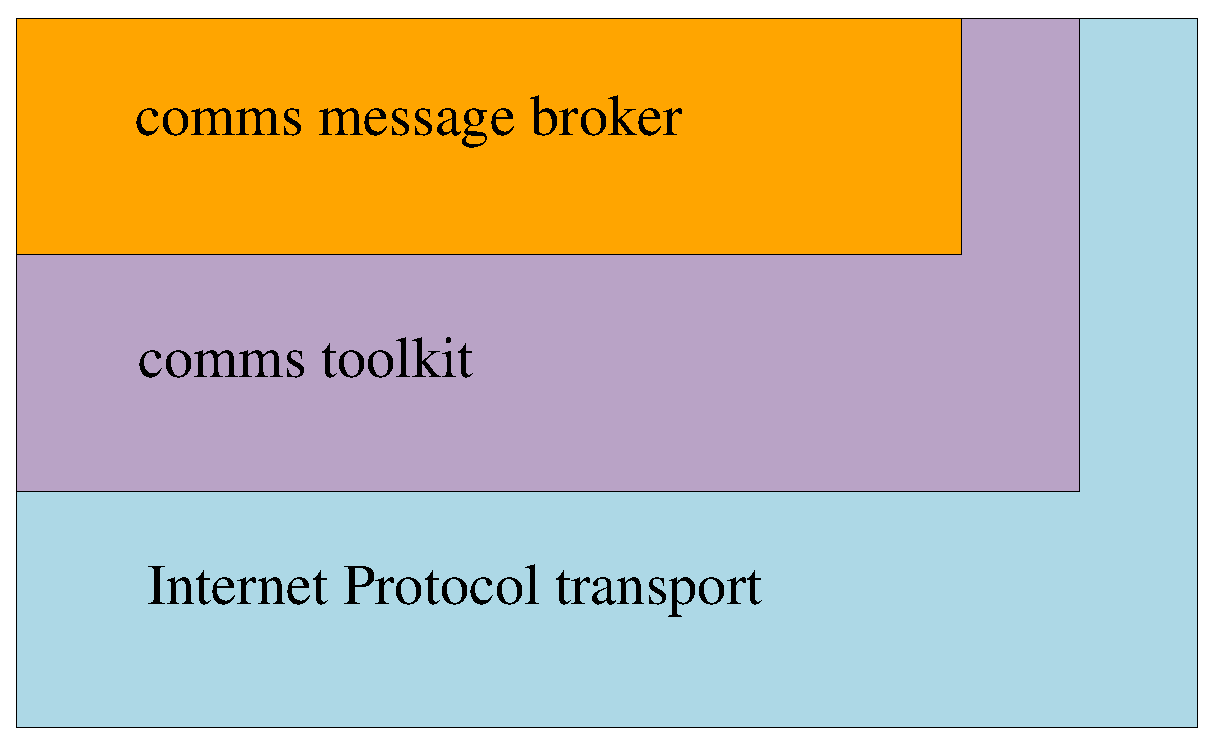
\includegraphics[scale=0.20]{comms}
\end{center}
\begin{itemize}
  \item{Layering is not rigid\\
        \ngrm\ components not overly constrained}
  \item{Bottom two layers are mostly off-the-shelf}
  \item{Generality reflects early phase of project in which it was conceived}
\end{itemize}
}\end{slide}
% ==========================================================================
\begin{slide}{Internet Protocols and Services}{\small
\begin{itemize}
  \item{Fully routed IP networks, e.g. route cluster management
	ethernets and IP-over-IB together}
  \item{Dynamic IP assignment, including multicast}
  \item{Private DNS, each session has a name, e.g. {\tt s2.s400.\ngrm.}}
  \item{Possibility for VPN isolation between jobs}
\end{itemize}
}\end{slide}
% ==========================================================================
\begin{slide}{Comms Toolkit}{\small
\begin{center}
  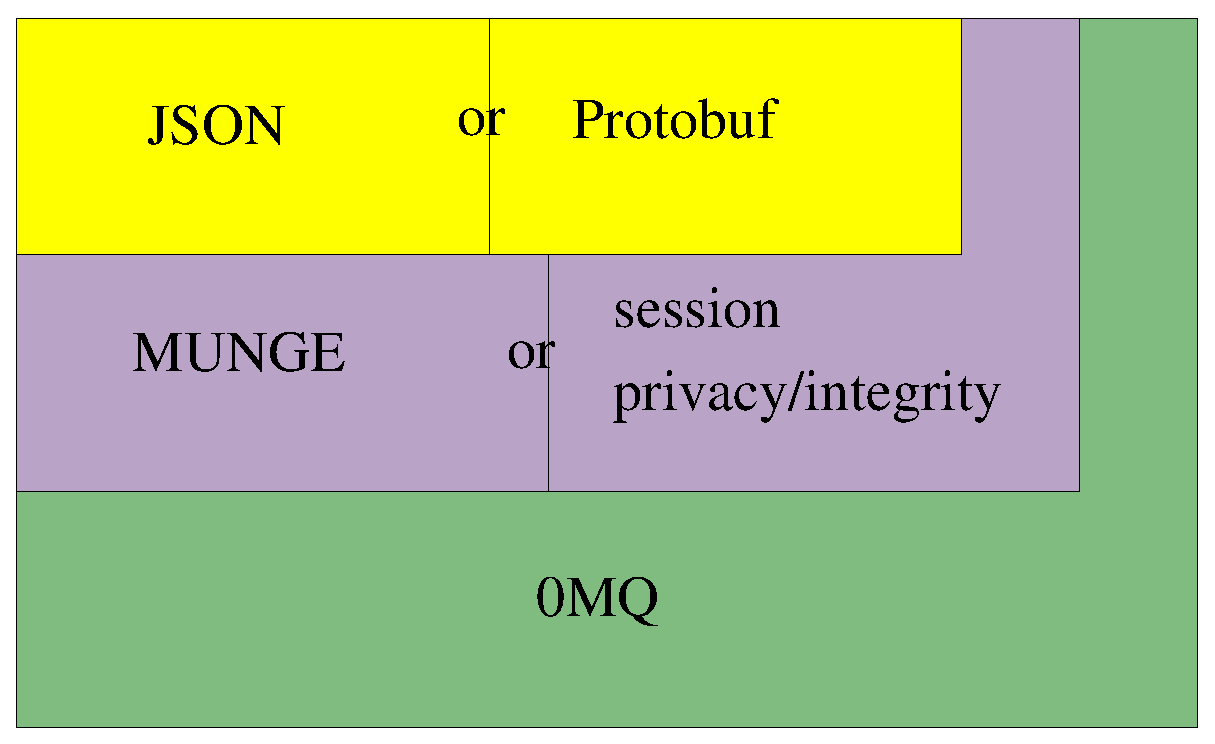
\includegraphics[scale=0.20]{commstk}
\end{center}
\begin{itemize}
  \item{Message handling (2 options)}
  \item{Security (2 options)}
  \item{Message encoding (2 options)}
\end{itemize}
}\end{slide}
% ==========================================================================
\begin{slide}{Message Handling}{\small
  \hfill
  \begin{minipage}{0.5\textwidth}
  {\bf \zMQ}
  \begin{itemize}
    \item{req-rep, pub-sub, push-pull}
    \item{PGM (reliable multicast)}
    \item{multipart message handling}
    \item{support for broker construction}
    \item{user space library}
  \end{itemize}
  \begin{center}
    \begin{minipage}[b]{0.15\linewidth}
    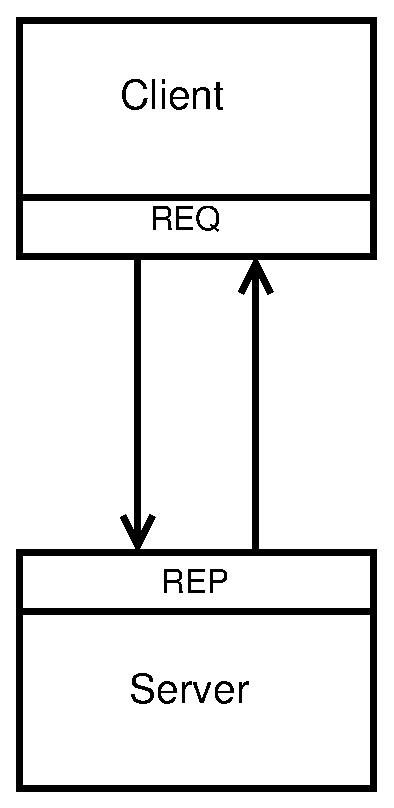
\includegraphics[scale=0.08]{comms_zmq_reqrep}
    \end{minipage}
    \hspace{0.2cm}
    \begin{minipage}[b]{0.3\linewidth}
    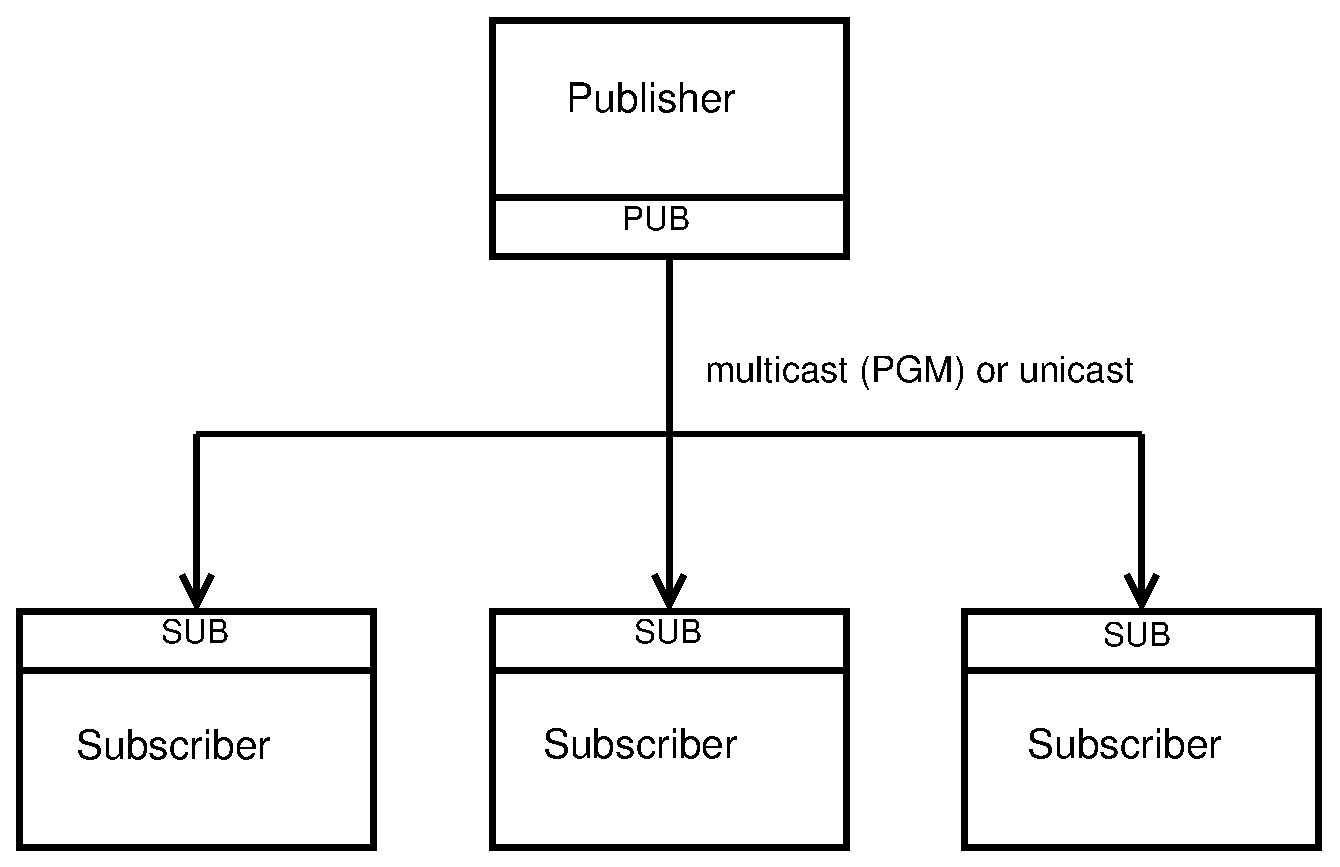
\includegraphics[scale=0.08]{comms_zmq_pubsub}
    \end{minipage}
    \hspace{0.2cm}
    \begin{minipage}[b]{0.3\linewidth}
    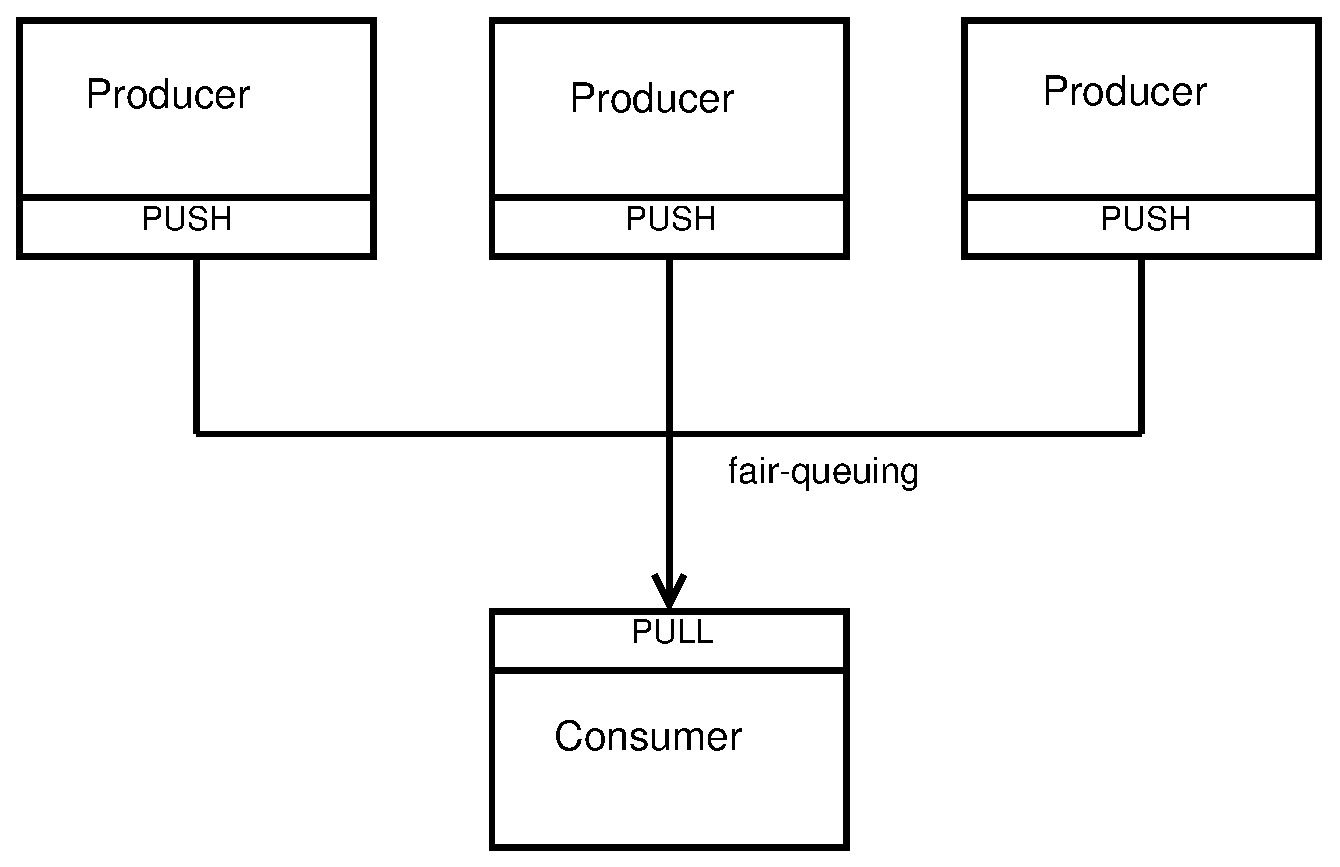
\includegraphics[scale=0.08]{comms_zmq_pushpull}
    \end{minipage}
  \end{center}
  \end{minipage}
  \hfill
  \begin{minipage}{0.45\textwidth}
  {\bf SCTP}
  \begin{itemize}
    \item{message oriented}
    \item{transparent multi-homing}
    \item{multi-streaming}
    \item{N-to-1 associations}
    \item{HMAC check option}
    \item{IETF, in Linux kernel}
  \end{itemize}
  \begin{center}
  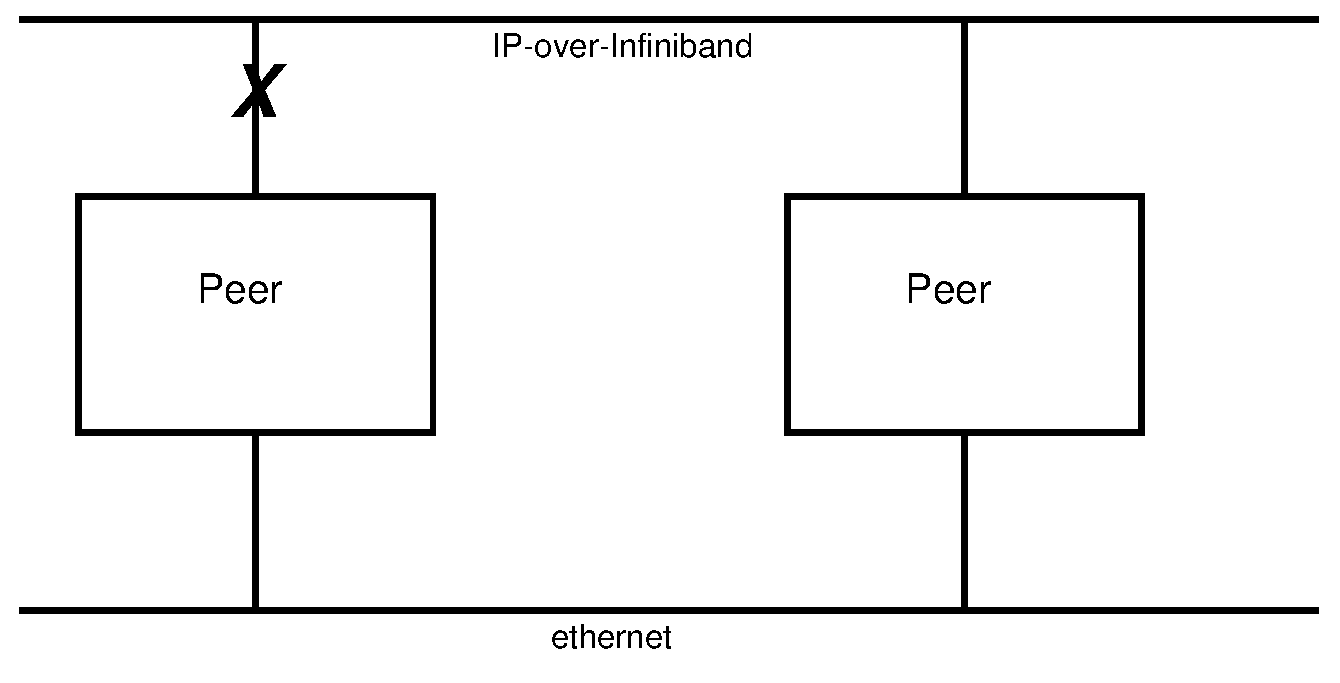
\includegraphics[scale=0.10]{comms_sctp}
  \end{center}
  \end{minipage}
  \hfill
}\end{slide}
% ==========================================================================
\begin{slide}{Security}{\small
  \hfill
  \begin{minipage}{0.5\textwidth}
  {\bf session security context}
  \begin{itemize}
    \item{key assigned by parent}
    \item{integrity, privacy for all}
    \item{parent knows child's key}
    \item{child forgets parent's key}
    \item{useful for pub-sub}
    \item{assumes trust within session}
  \end{itemize}
  \end{minipage}
  \hfill
  \begin{minipage}{0.45\textwidth}
  {\bf MUNGE}
  \begin{itemize}
    \item{key assigned out of band (don't ask)}
    \item{privileged munge daemon signs messages}
    \item{authenticates sender}
    \item{integrity, privacy of payload possible}
  \end{itemize}
  \end{minipage}
  \hfill
}\end{slide}
% ==========================================================================
\begin{slide}{Message Encoding}{\small
  \hfill
  \begin{minipage}{0.5\textwidth}
  {\bf JSON}
  \begin{itemize}
    \item{generated on the fly}
    \item{many language bindings}
    \item{human readable}
    \item{easily extended}
    \item{space-inefficient}
    \item{slow}
  \end{itemize}
  \end{minipage}
  \hfill
  \begin{minipage}{0.45\textwidth}
  {\bf Protocol Buffers}
  \begin{itemize}
    \item{compiled from IDL}
    \item{fewer supported languages}
    \item{machine readable}
    \item{must design for revision}
    \item{space-efficient}
    \item{fast}
  \end{itemize}
  \end{minipage}
  \hfill
}\end{slide}
% ==========================================================================
\begin{slide}{Comms Message Broker (CMB)}{\small
}\end{slide}
% ==========================================================================
\begin{slide}{Reduction Network}{\small
}\end{slide}
% ==========================================================================
\part{resource management}
\part{scheduler}
\part{monitoring}
\part{runtime}
% ==========================================================================
\end{document}
